\documentclass[11pt, a4paper, USenglish]{article}

\usepackage{modsim}



\begin{document}

% Titlepage
\title{TTK4145 - Compendium}
\author{Sander Furre}
\date{\today}
\begin{titlepage}
    \maketitle
    \begin{figure}
    \centering
    
\includegraphics[width=0.5\textwidth]{figures/misc/ie_logo.pdf}\\
    \end{figure}
    \thispagestyle{empty}
\end{titlepage}

% Contents
\part{Software quality}
\newpage
\part{Fault tolerance}
\section{Learning Goals:}
\begin{itemize}
    \item Understand/use: Reliability. Failure, fault, error. Failure Modes. Acceptance Test. Fault prevention vs. fault tolerance. Redundancy. Redundancy, static vs. dynamic. Forward/Backward error recovery
    \item Understand/use/evaluate techniques: N-version programming. Recovery blocks. Error detection. Failure mode merging. Acceptance tests 
\end{itemize}

\section{Reliability, Failure and faults}
There are 4 sources of faults in embedded systems
\begin{enumerate}
    \item Inadequate specification, i.e. misunderstanding the interactions between the program and the environment.
    \item Design errors in software components.
    \item Failure of hardware components. 
    \item Interference in the supporting communication subsystem.
\end{enumerate}

\textbf{Reliability} is a measure of the success with which the system conforms to some specification of its behavior. \textbf{Failure} is when the behavior of the system deviates from that which is specified for it. It in other words fail to follow specification. \textbf{Errors} are unexpected problems internal to the system which eventually manifests themselves in system's external behavior. \textbf{Faults} are the mechanical or software-related cause of failure. A failure in one (sub)system can cause faults in other systems:

\begin{figure}[H]
\centering
    Fault $\xrightarrow{\text{activation}}$ Error $\xrightarrow{\text{propagation}}$ Failure $\xrightarrow{\text{causation}}$ Fault
\end{figure}
Fault types
\begin{itemize}
\item Transient faults: Occur at some point in time, then disappear at some later point in time. E.g. hardware response to external electromagnetic field, fault disappears when the field disappears. Common kind of fault in communication systems.
\item Permanent faults: Occur at some point in time, lasts indefinitely until repair. E.g. software design faults.
\item Intermittent faults: Transient faults that sometimes happen and sometimes not. E.g. fault due to heat on heat sensitive hardware component.
\end{itemize}

Software faults are also called Bugs and we have two types:
\begin{itemize}
\item Bohrbugs: Reproducible, usually identifiable. Can be found and fixed with testing usually or diversity techniques.
\item Heisenbugs: Only activate under certain unknown, rare circumstances. Usually not found during testing. E.g. code shared between concurrent tasks that is not properly synchronized. Causes can be software ageing i.e. not freeing allocated memory. 
\end{itemize}

\subsection{Failure modes}
In short, failure modes describe the ways a (sub)system can fail.

We have two general classes of failure modes
\begin{itemize}
\item Value failure: Error in the value associated with service. Can be the result of a data conversion for example. The two categories are:
\begin{itemize}
    \item Constraint error: A fault causes a constraint to be breached.
    \item Value error: A fault causes a value to be incorrect.
\end{itemize}
\item Time failure: Service not delivered at the correct time. The thee categories are:
\begin{itemize}
    \item Too early
    \item Too late (Performance error)
    \item Infinitely late (Omission error)
\end{itemize}
\end{itemize}
Combination is called arbitrary failures. We also have \textbf{Commission/Impromptu} failure which describes a situation where a service delivered is not expected.

\begin{figure}[H]
\centering
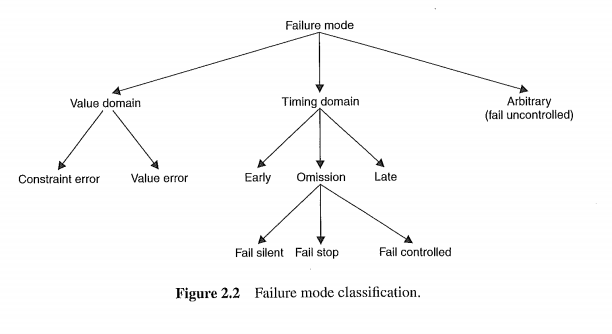
\includegraphics[width=0.5\textwidth]{figures/Fault_Tolerance/failure_mode_classification.PNG}
\end{figure}

Based on these failure modes we can sum up how the system might fail.
\begin{itemize}
\item Fail uncontrolled: Arbitrary or impromptu errors
\item Fail late: delivers service too late
\item Fail silent: Omission failure
\item Fail stop: Omission failure, but other systems can detect it.
\item Fail controlled: fails in a specified controlled manner.
\item Fail never: Self-explanatory.
\end{itemize}

\section{Fault prevention and fault tolerance}
\textbf{Fault prevention} aims to eliminate any and all faults before the system goes into operation, whilst \textbf{fault tolerance} enables the system to continue functioning even in the presence of faults. Both approaches attempt to give the system well-defined failure modes.

\subsection{Fault prevention}
Consists of two stages;
\begin{itemize}
\item Fault avoidance - Achieved by choosing reliable components, eliminating interference, having a complete requirements specification, following strict design methodologies and using languages with data abstraction and modularity, like Ada and Java.
\item Fault removal - Removing causes of errors mainly by system testing. Note that system testing is difficult. 
\end{itemize}
Any system will fail eventually either in hardware or software, and for real-time systems we therefore need fault tolerance.

\subsection{Fault tolerance}
Three levels of fault tolerance
\begin{enumerate}
\item \textbf{Full fault tolerance} - The system continues to operate in the presence of faults for a limited time period with no significant loss of functionality or performance. Required in most safety-critical systems in theory.
\item \textbf{Graceful degradation} - also known as fail soft. The system continues to operate in presence of errors, accepting a partial degradation of functionality or performance until recovery or repair. Safety-critical systems often settle for this type of fault tolerance in practice. Graceful degradation necessity for applications with high availability requirements.
\item \textbf{Fail safe} - The system maintains its integrity while accepting temporary halt in  its operation. In other words, it shuts down safely temporarily to allow for maintenance. 
\end{enumerate}

The goal of fault tolerance is to minimize redundancy while maximizing reliability subject to cost, size and power constraints of the system.

\begin{figure}[H]
\centering
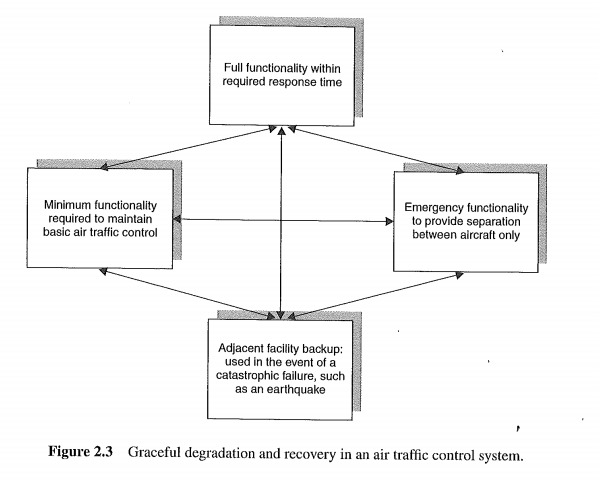
\includegraphics[width=0.5\textwidth]{figures/Fault_Tolerance/graceful_degradation_example.PNG}
\end{figure}

\subsection{Redundancy}
\textbf{Protective redundancy} introduces components that detects and recovers
the systems from faults, but are unnecessary for normal operation. When
designing a fault-tolerant system, the goal is to minimize redundancy while
maximizing reliability, subject to constraints on cost, size and power consumption. The redundant components can (and will) increase complexity, and it is useful to separate them from the rest of the system.
We separate between static and dynamic redundancy, both for hardware
and software. First, let’s have a look at hardware redundancy:

\begin{itemize}
\item Static redundancy (or masking) is based on redundant components
“hiding” faults. An example is Triple Modular Redundancy (TMR),
where a majority voting circuit is used. The output of three identical
components are compared, and if one differs from the others, its output
is masked out. It is assumed that faults are transient.
\item Dynamic redundancy is an error-detection facility within a component, making it possible for that component to indicate if its output is
in error. Note that the component does not hide or fix the error, that
must be done by some other part of the system. Examples are checksums (see parity byte section on Wikipedia for very simple example) and parity bits. 
\end{itemize}

For fault tolerance with regards to software design, we have \textit{N-version programming} which works like masking, and \textit{error detection and recovery}.
The latter is dynamic redundancy in the sense that recovery is only brought
into action once an error has occurred.

\section{N-version programming}
From one initial specification, N independent programs are created. In operation, they run concurrently, and their outputs are compared by a driver process. The “correct” result is determined by majority of vote, like with masking. 

Assumption: Program can be completely, consistently and unambiguously specified and independently developed programs will fail independently.

Example: On Boeing 777 flight control system, single Ada program was produced  but three different processors and three distinct compilers were used to obtain diversity.

The driver process invokes the versions, waits for completion of voting, compares results and acts on these results.

\begin{figure}[H]
\centering
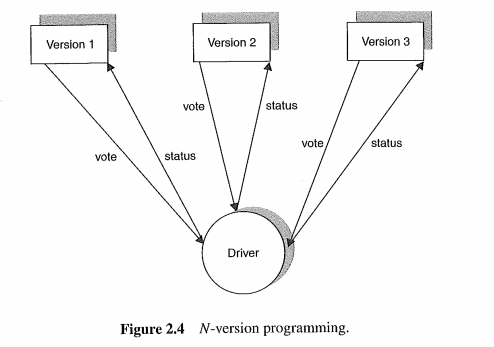
\includegraphics[width=0.5\textwidth]{figures/Fault_Tolerance/N_version_programming.PNG}
\end{figure}

In the context of embedded systems, we check the versions underway and not at the end. Interaction between the driver and the versions consists of 3 components
\begin{enumerate}
\item Comparison vectors: Also called votes, consists of output and metadata (attributes)
\item Comparison status indicators: Commands from driver. Indicates the actions that each version must perform as result of comparison. Can be \textit{continuation}, \textit{termination} or \textit{continuation with vote modification} on some of the versions.
\item Comparison points: The points in the code where votes must be communicated to the driver process.
\end{enumerate}

Challenges concerning N-version programming are:
\begin{itemize}
\item \textbf{Initial specification} - A specification error will manifest itself in all N versions of the implementation.
\item \textbf{Independence of design effort} - The assumption that versions will fail completely independently of each other is not reality in practice.
\item \textbf{Adequate budget} - N-version programming technique can require N times the budget of a 1 version technique.
\end{itemize}

\section{Software dynamic redundancy}
With dynamic redundancy, the redundant components only come into operation when an error manifests itself. There are four phases to dynamic redundancy in software:
\begin{enumerate}
\item \textbf{Error detection} - Most faults will manifest themselves in form of an error. No Fault tolerance scheme can be utilized until the error is detected.
\item \textbf{Error diagnosis} - There is a delay between a fault becoming active and error detection, the propagation of erroneous information in the system is assessed.
\item \textbf{Error recovery} - Transform the corrupted system into a state form which it can continue its normal operation (perhaps with degraded functionality).
\item \textbf{Fault treatment} - Maintenance must be performed to correct the underlying fault responsible for the error.

\end{enumerate}

\subsection{Error detection}
There are two classes:
\begin{itemize}
\item \textbf{Environmental detection} - Detection by hardware or run-time support system. E.g. overflow error in hardware or out-of-bounds error for array in run-time)
\item \textbf{Application detection} - Detect error with application specific code.
\begin{itemize}
    \item \textbf{Replication checks} - N-version programming with N=2
\item \textbf{Timing checks} - Watchdog or deadline checks
\item \textbf{Reversal checks} - Calculate input from output and check for match.
\item \textbf{Coding checks} - Test for corruption of data. Based on redundant data, i.e. checksum.
\item \textbf{Reasonableness checks} - Are based on knowledge of the internal design and construction of the system. I.e. range violation and assertions.
\item \textbf{Structural checks} - Metadata about structures
\end{itemize}
\end{itemize}
Note that all forms of application detection mentioned can be implemented in hardware and are then considered to be environmental detection.

\subsection{Error diagnosis}
Software designers aim to minimize the damage caused by a faulty component, this is called firewalling. Two techniques are:
\begin{itemize}
\item \textbf{Modular decomposition} - Modules only communicate through well defined interfaces, internal details are hidden. Provides a static structure.
\item \textbf{Atomic actions} - are indivisible, and appear to happen instantaneously for the rest of the system. Often called \textbf{transactions} or atomic transactions. They are used to move the system from one consistent state to another, and limit the flow of information between components/modules.
\end{itemize}

\subsection{Error recovery}
The two approaches here are forward and backward error recovery.
\begin{itemize}
\item \textbf{Forward Error Recovery} - Attempts to continue from the corrupted state by making selective corrections to the state.
\item \textbf{Backward Error Recovery} - Relies on restoring the system to a safe state previous to that in which the error occurred. This safe state is called an recovery point and the act of establishing it is called \textbf{checkpointing}.
\end{itemize}

Advantage of backward error recovery is that it does not rely on finding the location or cause of faults. Can therefore be used to recover from unanticipated faults including design errors. A disadvantage on the other hand is that it cannot undo effects the fault may have had on the environments (missile launch) and it can be time-consuming. Another disadvantage is the possibility of the domino effect.

\textbf{The domino effect} is a possible issue in state restoration with concurrent processes. Consider the following scenario in Figure \ref{fig: domino_effect}. 

\begin{figure}[H]
\centering
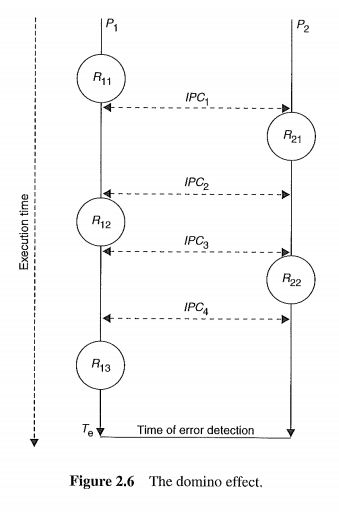
\includegraphics[width=0.5\textwidth]{figures/Fault_Tolerance/domino_effect.PNG}
\label{fig: domino_effect}
\end{figure}

If P1 detects an error at Te then it is simply rolled back to R13. If on the other hand P2 detects an error at Te it is rolled back to R22 and thus must undo IPC4. This means that P1 must be rolled back to R12 which means it must undo IPC3 which means P2 must rollback to R21 and undo IPC2 and so on. Potentially the two processes have to be rolled back to the beginning of their interaction. The only way to be guaranteed to stop this is with \textbf{recovery lines} which are consistent set of recovery points across all processes that communicates together.

\section{Recovery blocks and acceptance tests}
Recovery blocks are normal blocks in the programming language sense but where the entrance is an automatic recovery point and the exit an acceptance test. 
\begin{figure}[H]
\centering
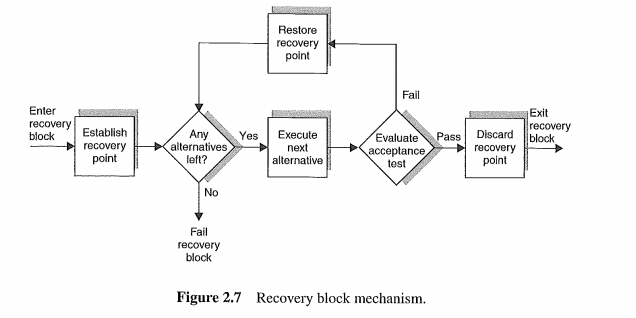
\includegraphics[width=\textwidth]{figures/Fault_Tolerance/recovery_block_mechanism.PNG}
\end{figure}

\subsection{Acceptance test}
The acceptance test is used to test that system is in an acceptable state after the execution of the block (also called primary module). If it fails program is restored to recovery point at beginning of block and an alternative module is being executed. If all alternative modules fail the block fails.

One should keep in mind the tradeoff between comprehensive testing and keeping overhead at a minimum. All error detection techniques mentioned earlier may be used as acceptance tests.

\subsection{Comparison between N-version programming and recovery blocks}
\begin{itemize}
\item \textbf{Static vs. Dynamic}-version is static because all versions run all the time. Recovery blocks are dynamic because the alternative code only runs when acceptance test fails.
\item \textbf{Associated overhead} - Both methods increase overhead/complexity.
\item \textbf{Diversity of design} - Both exploit this and are therefore susceptible to errors that originate in the specification.
\item \textbf{Error detection} - N-version uses vote and recovery blocks uses acceptance test. Exact voting less overhead than acceptance testing. Same cannot be concluded for inexact voting.
\item \textbf{Atomicity} - Backward error recovery criticized because cannot undo effects or damage which may have occurred in the environment. N-version programming avoids this because all versions are assumed to not interfere with each other; they are atomic. They communicate only with the driver through voting. Not that it is possible to structure program such that unrecoverable operations do not occur in recovery blocks.

Note that N-version programming and recovery blocks can be considered competing techniques, but also complementary techniques.
\end{itemize}

\section{Dynamic redundancy and exceptions}


The goal if this section is to introduce framework for implementing software fault tolerance based on dynamic redundancy and the notion of exceptions and exception handlers.

An \textbf{exception} is the occurrence of an error. \textbf{Raising} (or throwing or signaling) an exception is bringing the exception condition to the attention of the invoker of the operation which caused the exception. In less formal wording, this means letting the program know an error has occurred. \textbf{Handling} (or catching) an exception is the invoker's response to the raised exception.

Note that exception handling is a forward error recovery mechanism, but it can also be used to provide backward error recovery.

\begin{figure}[H]
\centering
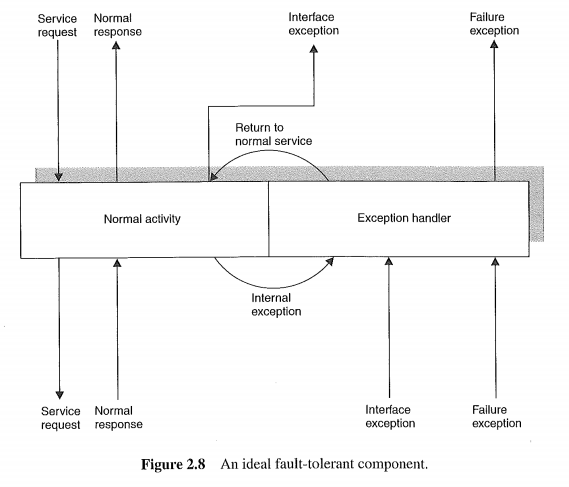
\includegraphics[width=\textwidth]{figures/Fault_Tolerance/ideal-fault-tolerant-component.PNG}
\end{figure}




\newpage
\part{Fault model and software fault masking}
\newpage
\part{Transaction fundamentals}
\textit{Disclaimer: This part is not very good pedagogically. It is unclear what the context is for the terminology and methodology used. It seems to be based around JAVA infrastructure or something. The notes I have therefore are unable to give any decent intuition and are more used as a high-level explanatory thingy for when questions regarding this appears on exams.}

\section{Learning Goals}
\begin{itemize}
\item Knowledge of eight “design patterns” (Locking, Two-Phase Commit, Transaction Manager, Resource Manager, Log, Checkpoints, Log Manager, Lock Manager), how they work and which problems they solve. Ability to utilize these patterns in high-level design. 
\item Comprehension of terms: Optimistic Concurrency Control, Two-phase commit optimizations, Heuristic Transactions, Interposition.
\end{itemize}

\section{Motivation and context}
\begin{itemize}
\item We need error handling and containment for systems with multiple participants (threads, processes, distributed systems). These participants must often cooperate in the error handling.
\item Transactions (and atomic actions) are techniques/frameworks that provide the means to do this. They fall under the category of dynamic SW redundancy. 
\item Transactions contribute towards the desired error assessment and confinement design and help avoid the \textit{domino effect}
\end{itemize}

We will learn Transaction fundamentals through \textbf{eight design patterns} and some additional terms. Before we get into that note that a transaction is an indivisible, atomic action with backward error recovery. The properties of a transaction described by \textit{ACID properties}
\begin{itemize}
\item \textbf{Atomicity} -  The transaction either commits successfully or aborts completely.
\item \textbf{Consistency} - Transactions preserve a consistent state.
\item \textbf{Isolation} - Intermediate states during a transaction are not visible from the outside. Furthermore, transactions appear to be executing serially even when they are not.
\item \textbf{Durability} - The effects of a commited transition are never lost, they are stored in stable storage such as a hard drive.
\end{itemize}

With backward error recovery the flow of control of a single-threaded program is as follows:
\begin{verbatim}
allocate locks
create recovery point
do work(goto end if any problems)
label end:
if (error) {
	roll back to recovery point
    status=FAIL
} else {
    status=OK
}
release locks
return status
\end{verbatim}
It should be noted that the acceptance test that is responsible for detecting the errors in the program above.

The workings of a transaction can be further visualized by a sequence diagram. It can be a good idea to read about the eight design patterns and come back to this figure. 
\begin{figure}[H]
\centering
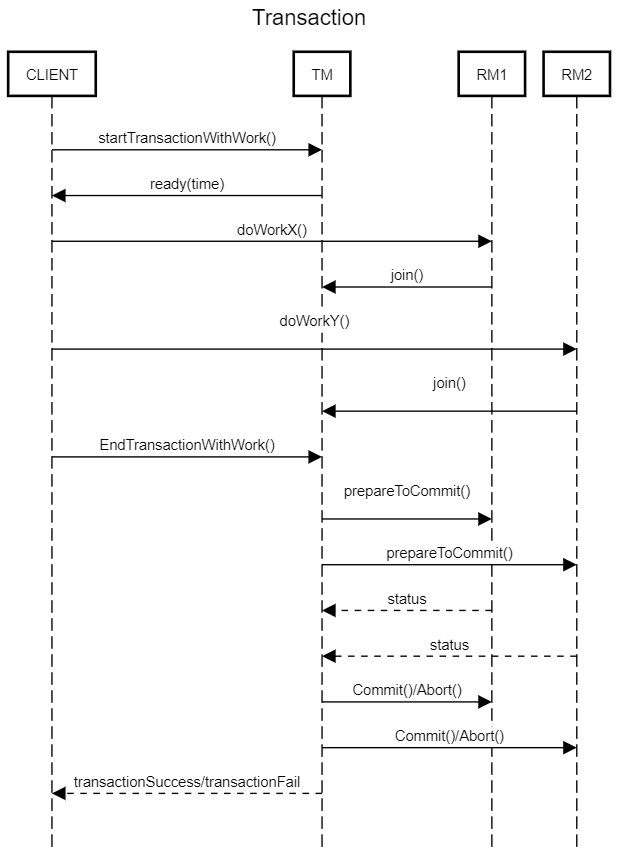
\includegraphics[width=0.6\textwidth]{figures/Fault_Tolerance/TransactionSequence.png}
\end{figure}

\section{The 8 design patterns}
\subsection{Two-phase commits}
Associated with each transaction is a coordinator/Transaction Manager, that communicates with the participants. The message flow is as follows:
\begin{verbatim}
Coordinator                                          Participant
                             QUERY TO COMMIT
                 -------------------------------->
                             VOTE YES/NO             prepare*/abort*
                 <-------------------------------
commit*/abort*               COMMIT/ROLLBACK
                 -------------------------------->
                             ACKNOWLEDGMENT          commit*/abort*
                 <--------------------------------  
end
\end{verbatim}
\subsubsection{Basic Algorithm}
Commit request (or voting) phase 
\begin{enumerate}
\item Coordinator sends \textbf{query to commit} and waits until has received reply from all participants
\item Participants execute transaction up to the point where they will be asked to commit. Each write entry to undo lo and redo log.
\item Participants vote \textbf{Yes} if their actions succeeded or \textbf{No} if they have experienced a failure making it impossible to commit.
\end{enumerate}
Commit/Completion phase
\begin{itemize}
\item \textbf{Success} - All participants voted yes. Coordinator responds with commit instruction.
\item \textbf{Failure} - At least one participant voted no. Coordinator responds with rollback instruction.
\end{itemize}

Note that: A disadvantage with two-phase commits is that the protocol is blocking. Participants will block after they have voted, awaiting a commit or rollback
message. If the coordinator fails, they will never receive either.

\subsection{Locking}
Ensures that intermediate states are not propagated. Additionally, ensures that participants can only communicate with other participants. The participant must be part of the ongoing transaction to be able to use the locked resource. 

\subsection{Lock Manager}
Can have the following functionality:
\begin{itemize}
\item Release all locks associated with transaction X when it finishes.
\item Tidy up after restart (open locks that should be open etc.)
\item Handle resources shared by several Resource Managers.
\item Include deadlock avoidance and detection algorithms.
\end{itemize}
Can also have other functions relating to locks.

\subsection{Resource Manager}
The resource managers are the \textit{transaction participants}. 
\begin{itemize}
\item Keeps track of locks and recovery points
\item Communicates with transaction manager during voting and commit phases.
\end{itemize}

\subsection{Transaction Manager}
Useful if there are multiple participants
\begin{itemize}
\item Creates the transaction, keeps track of participants
\item Plays the role of coordinator
\item Can provide a transaction deadline and abort if the deadline is missed.
\end{itemize}

\subsection{The log}
\begin{itemize}
\item Alternative to checkpoints
\item Every participant including the TM writes every planned change of state to the log and waits until the operation is confirmed safe to perform it. 
\item Processes can restore state after restart by executing the logrecords.
\item Logrecords can be executed backwards to undo actions, therefore no need for checkpoints.
\end{itemize}

\subsection{The Log manager}
Queues logrecords, optimizes disk access and sends acknowledgments receipts on received log records.

\subsection{Checkpoints}
Discussed before, alternative to log method described above. Stores a consistent state that we can start the system in.

\section{Other terms}
\subsection{Optimistic concurrency control:}
This method assumes that multiple transactions can frequently complete without interfering with each other. While running, transactions use resources without utilizing locks or other synchronization primitives. This works because before committing, each transaction verifies that no other transaction has modified the data it has read. If conflicting modifications are revealed, the transaction is rolled back and restarted. OCC can work well when we have low data contention, meaning when conflicts are rare

\subsection{Two-phase commit optimizations}
Different methods exist here
\begin{itemize}
\item Early abort using e.g. ATC
\item One-phase when only one participant
\item Read-only operations will never be aborted thus will always yield commit.
\item Last resource commit: One participant gets to wait until all the other votes are in and take these into consideration before making its vote.
\end{itemize}

\subsection{Heuristic transactions}
What if we give our vote and then loose connection? We have to make local guess and maybe to forward error recovery after.

\subsection{Interposition}
The TM's ability to play the role of a RM.

\newpage
\part{Atomic actions}
\section{Learning goals}
\begin{itemize}
\item  A thorough understanding of the problems Atomic Actions are meant to solve and how these motivates the different aspects of Atomic Actions.
\item Ability to use and implement Atomic Actions, including the mechanisms providing the start, side and end boundaries.
\item Understanding the motivation for using Asynchronous Notification in Atomic Actions.
\item A coarse knowledge of how the mechanisms for Asynchronous Notification in C/Posix, ADA and Java works.
\end{itemize}

\section{What are atomic actions}
\subsection{Motivation for using atomic actions}
An Atomic Action is a design framework for damage confinement and error recovery. Before we go into the actual details, lets just give a heads up and say that a transaction discussed in the last part is in fact an atomic action structure with backward error recovery. We know from before that should have \textit{recovery line} to avoid domino effect if we have backward error recovery. The question is how we achieve synchronization of recovery points. With atomic actions, we get the structure necessary to achieve both backward and forward error recovery. The recovery synchronization is not a straight line here, it is a registration of when a task enters an atomic action and if something goes wrong within it, all tasks in it are rolled back to the state they were in when they entered the atomic action. The general usage of atomic cations is for when several groups of concurrent tasks need to be structured to allow for coordination of their activities. The \textbf{atomic action} is required for each group of tasks to execute their joint activity. It should be mentioned that a single task may also want to protect itself from interference from other tasks. Atomic actions can therefore be said to involve one or more tasks and be a method for structuring these tasks such that they can operate on different parts of a single task concurrently. Figure \ref{fig: atomic_actions} shows a simplistic representation of how atomic actions work.

\begin{figure}[H]
\centering
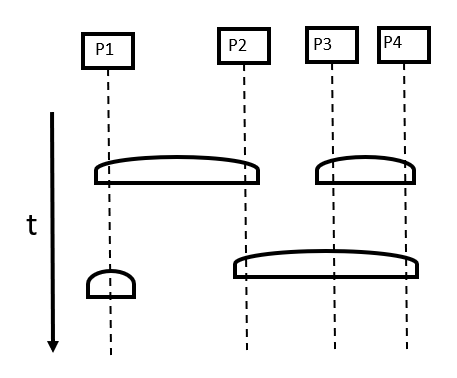
\includegraphics[width=0.6\textwidth]{figures/Fault_Tolerance/atomic_actions.PNG}
\label{fig: atomic_actions}
\caption{Illustration of how atomic actions can work}
\end{figure}

\subsection{Different ways to define atomic actions }
\begin{enumerate}
\item An action is atomic if the tasks performing it are not aware of the existence of any other active tasks, and no other active tasks is aware of the activity of the tasks during the time the tasks are performing the action. 
\item An action is atomic if the tasks performing it do not communicate with other tasks while the action is being performed.
\item An atomic action has tasks that cannot detect state change except those performed by themselves and they do not reveal their state changes until the action is complete.
\item Atomic actions are by other tasks considered to be indivisible and instantaneous such that the effects on the system are as if they were interleaved as opposed to concurrent.  
\end{enumerate}

\subsection{Requirements for atomic actions}
\begin{itemize}
\item \textbf{Well-defined boundaries} - Each atomic action should have a \textit{start}, an \textit{end} and a \textit{side boundary}. Start boundary is the location in each task involved in the atomic action where the action is deemed to start. The end boundary is where it is deemed to end and the side boundary separates tasks involved with the atomic action from those not involved.
\item \textbf{Indivisibility (isolation)} - an atomic action must not allow the exchange of any information between the tasks on each side of the side boundary. If two atomic actions share data trough a Resource Manager then the value is determined by strict sequencing. There is no implied \textit{synchronization} at the start of an atomic action, but tasks are not allowed to leave the atomic action until all tasks are willing and able to leave.
\item \textbf{Nesting} - Atomic actions may be nested as long as they do not overlap with other atomic actions. In general only \textit{strict nesting} allowed where one is completely contained within the other.
\item \textbf{Concurrency} - It should be possible to execute different atomic actions concurrently
\end{itemize}

\subsection{Standard Atomic Actions implementation}
Transaction mentioned in last part is a good example of an atomic action.
Start boundary:
\begin{enumerate}
\item Dynamic (call to e.g. \textit{startTransactionWithWork()}
\end{enumerate}
Side boundary:
\begin{enumerate}
\item Locking, no unlocking before safe state (end boundary).
\end{enumerate}
End boundary:
\begin{enumerate}
\item Vote counting (two-phase commit)
\item Synchronization primitive barrier that no one can pas through before everyone has arrived.
\end{enumerate}

\section{Language-specific atomic action implementation}
\todo{Fill out more here}
Java:
\begin{itemize}
\item Synchronized methods, wait, notify / notifyAll
\item Asynchronous exceptions
\end{itemize}
Ada:
\begin{itemize}
\item Protected objects
\item Function procedures and entries with guards.
\end{itemize}
C/POSIX
\begin{itemize}
\item pthread cancel
\item setjmp and longjmp
\end{itemize}

\section{Asynchronous notification}
Asynchronous notification is a bit like interrupts in hardware. It is a way to distribute error information instead of using the commit structure discussed or some polling regime to make forward error recovery possible instead of just backward error recovery. To get a recoverable action we must be able to get the attention of a task involved in the action that an error has occurred in another task involved in the action. This is achieved with an asynchronous notification mechanism which most programming languages and operating systems support. As with exceptions, there are two basic models; \textbf{resumption} and \textbf{termination}. 

\subsection{Resumption (event handling)}
Behaves like a software interrupt. A task indicates which events it is willing to handle; when the event is signaled the task is interrupted and an event handler is executed. Afterwards the task resumes from where it was when the interrupt came in.

\subsection{Termination model}
Each task specifies a domain of execution during which it is prepared to receive  an asynchronous notification that will cause the domain to be terminated. In less formal wording, this means that after we handle the error we terminate what we were doing and start somewhere else in the code, for example lower down.

\subsection{The user need for asynchronous notification}
Fundamental need is to enable tasks to respond \textit{quickly} to a condition which has been detected by another task. There are several occasions where polling for events or waiting for the event to occur is inadequate:
\begin{itemize}
\item \textbf{Error recovery} - When groups of tasks undertake \textit{atomic actions}, an error detected in one task requires all other tasks to participate in the recovery as the work they are now doing might be useless if the error has propagated. The form of asynchronous notification we will use here for termination is \textit{Asynchronous Transfer of Control (ATC)}
\end{itemize}

\subsection{Language specific asynchronous notification implementation}
\subsubsection{C/POSIX}
Supports the resumption model. Has a set of predefined signals and 3 ways in which a process can deal with a signal. 
\begin{enumerate}
\item \textbf{Block} - Handle it later or accept it
\item \textbf{Handle} - Setting a function to be called whenever it occurs
\item \textbf{Ignore} - The signal is simply lost
\end{enumerate}
If we want asynchronous transfer of control we can use \textbf{setjmp} and \textbf{longjmp} mechanisms. 
\begin{verbatim}
#include <stdio.h>
#include <setjmp.h>

static jmp_buf buf;

void second(void) {
    printf("second\n");			 	   // prints
    longjmp(buf,1); 				// jumps back to where setjmp was called
}

void first(void) {
    second();
    printf("first\n"); 					// does not print
}

int main() {
    if ( ! setjmp(buf) ) {
        first(); 								 // when executed, setjmp returns 0
    } else { 									// when longjmp jumps back, setjmp returns 1
        printf("main\n"); // prints
    }
    return 0;
}
\end{verbatim}
When program above executed it will return "second main"

\subsubsection{Asynchronous notification in Ada}
The asynchronous notification facilities in Ada allow an application to respond to among other things asynchronous transfer of control (ATC) requests on a task - supporting a termination model. There is no generalized model for resumption in Ada. To emphasize that ATC is a form of communication and synchronization, the mechanism  is built on top of the inter-task communication facility.

We will look at of \textit{Asynchronous select} here. 
\newpage
\begin{lstlisting}
select
    Trigger.Event;
    -- optional sequence of statements to be 
    -- executed after the event has been received
then abort
    -- abortable sequence of statements
end select;
\end{lstlisting}
It is best explained with an example
\begin{lstlisting}
task Server is
	entry ATC_EVENT;
end Server;

task To_Be-Interrupted;

task body Server is
begin
	...
    accept ATC_EVENT do 
    	Seq2; 
    end ATC_EVENT;
    ...
end Server;

task body To_Be_Interrupted is
begin
	...
    select -- ATC statement
    	Server.ATC_EVENT;
        Seq3;
    then abort
    	Seq1; 
        -- the work here is the normal operation work
        -- Will be interrupted if it times out or event happens
    end select;
    Seq4;
    -- Seq4 comes after the asynchronous select, it cannot be interrupted.
    ...
end To_Be_Interrupted;
\end{lstlisting}
When the above ATC statement is executed, the statements which are executed will depend on the order of events that occur. See page 257 in BW chapter 7. The Ada ATC facility described above is used to implement both forward and backward error recovery.

\newpage

\subsubsection{Asynchronous notification in Java}
ATC here also. Focus on Real-Time Java.
\begin{itemize}
\item Built on Java exceptions
\item Can be blocked
\end{itemize}





\newpage
\part{Modeling of concurrent programs}
\section{Learning Goals}
\begin{itemize}
\item An understanding of how using message-based synchronization leads to a very different design than shared variable synchronization.
\item Model, in FSP and by drawing transition diagrams, simple programs (semaphore-based or message-passing).
\item Draw very simple compound (for parallel processes) transition diagrams.
\item  Sketch simple message-passing programs.
\item An understanding of how using message-based synchronization leads to fewer transition-diagram states than shared variable synchronization.
\item Understanding the terms deadlock and livelock in context of transition diagrams
\end{itemize}

\section{Modeling}
Classic deadlock example:
\begin{verbatim}
T1:
    while (1) {
        Wait(A)
        Wait(B)
        ...
        Signal(A)
        Signal(B)
    }
T2:
    while (1) {
        Wait(B)
        Wait(A)
        ... 
        Signal(B)
        Signal(A)
    }
\end{verbatim}
Let us introduce \textbf{processes} and \textbf{events}. All processes that 'care about' an event experience it at the same time. For modeling we use FSP (Finite State Processes) $\subset$ CSP (Communicating Sequential Processes). Note that Ada \texttt{entries} can be modelled as events. \todo{The last few sentences don't make much sense, improve}. For message-based systems (message passing, synchronous communication), modeling with processes, events and guards comes naturally. Some explanation of symbols before we get into the next part. The numbers below in the diagrams are the \textbf{states}. In the textual representation these are \textbf{arrows.} The text such as $t1sa$ is an event. What this means is that to get for example an $t1sa$ event, T1 has to be in state 3 and SA has to be in state 2. Check the diagrams below, this is a bit tricky but makes sense.
\begin{verbatim}
    T1 = (t1wa -> t1wb -> t1sb -> t1sa -> T1).
    T2 = (t2wb -> t2wa -> t2sa -> t2sb -> T2).
\end{verbatim}
\begin{figure}[H]
\centering
\begin{subfigure}{.5\textwidth}
\centering
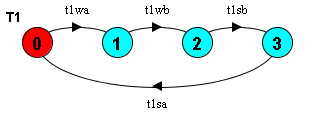
\includegraphics[width=.9\linewidth]{figures/Modeling concurrent programs/Example1/T1.PNG}
\end{subfigure}%
~
\begin{subfigure}{.5\textwidth}
\centering
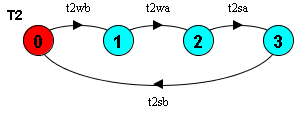
\includegraphics[width=.9\linewidth]{figures/Modeling concurrent programs/Example1/T2.PNG}
\end{subfigure}
\end{figure}

No deadlock is visible here, we need to model the semaphores:
\begin{verbatim}
    SA = (t1wa -> t1sa -> SA | t2wa -> t2sa -> SA).
    SB = (t1wb -> t1sb -> SB | t2wb -> t2sb -> SB).
\end{verbatim}
\begin{figure}[H]
\centering
\begin{subfigure}{.5\textwidth}
\centering
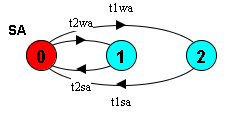
\includegraphics[width=.9\linewidth]{figures/Modeling concurrent programs/Example1/SA.PNG}
\end{subfigure}%
~
\begin{subfigure}{.5\textwidth}
\centering
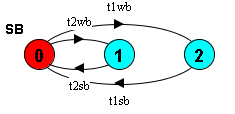
\includegraphics[width=.9\linewidth]{figures/Modeling concurrent programs/Example1/SB.PNG}
\end{subfigure}
\end{figure}
To model the complete, concurrent/parallel system:
\begin{verbatim}
    ||SYSTEM = (T1 || T2 || SA || SB).
\end{verbatim}
\begin{figure}[H]
    \centering
    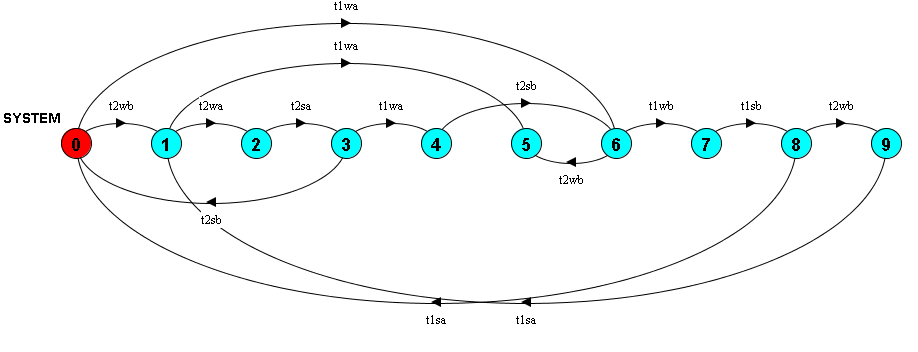
\includegraphics[width=\linewidth]{figures/Modeling concurrent programs/Example1/SYSTEM.PNG}
\end{figure}
In a \textbf{transition diagram}, a deadlock is a state with no exit. Such a state can be observed in the figure above in state 5. A livelock is a subset of states we cannot exit. 
\begin{verbatim}
LL = (s1 -> LOOP), LOOP = (s2 -> s3 -> LOOP).
\end{verbatim}
\begin{figure}[H]
\centering
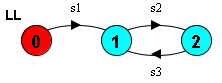
\includegraphics[width=0.5\linewidth]{figures/Modeling concurrent programs/LiveLock/LiveLock.PNG}
\end{figure}
Before mentioning the Dining philosophers problem, have a look at this basic code producing a deadlock
\begin{verbatim}
MOVE = (north->(south->MOVE|north->STOP)).
\end{verbatim}
\begin{figure}[H]
\centering
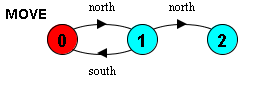
\includegraphics[width=0.5\linewidth]{figures/Modeling concurrent programs/Deadlock/Deadlock.PNG}
\end{figure}
Dining philosophers with deadlock is shown next
\begin{verbatim}
    FORK = (get -> put -> FORK).
    PHIL = (sitdown -> right.get -> left.get -> eat ->
            right.put -> left.put -> arise -> PHIL).
    
    || DINERS(N=5) = forall [i:0..N-1]
            (phil[i]:PHIL ||
            {phil[i].left, phil[(i-1+N)%N].right}::FORK).
\end{verbatim}
Some advance syntax is used here:
\begin{itemize}
    \item \texttt{phil[i]:PHIL} exchanges \texttt{eat} with \texttt{phil1.eat}, and thus takes care of all events for all N philosophers.
    \item \texttt{{phil[i].left, phil[(i-1+N)\%N].right}} means that either of the two options in curly braces are possible.
    \item \texttt{{phil[i].left, phil[(i-1+N)\%N].right}::FORK} then means that either \texttt{phil[i].left.get} or \texttt{phil[(i-1+N) mod N].right.get} are possible for the same fork, i.e. it can be picked up by the philosopher to its right or left.
\end{itemize}
Transition diagram is huge, needs an analyzing tool such as the infamous LTS Analyzer to find the deadlock potential! Some notes on the Dining Philosophers problem:
\begin{itemize}
\item If we make some of the philosophers left-handed the deadlock is avoided. But hugely unfair as one philosopher next to the one causing the deadlock would have to finish his meal before the other philosopher gets both his forks. \textit{This is not very well explained, sorry but I don't have a philosopher's stone that makes me godly enough to explain this well}
\item A a resource hierarchy on the forks, where the philosophers would always pick up the lowest value fork first could improve fairness. \textit{It is far beyond the scope of this compendium, this course, my sanity or the universe itself to properly explain why}
\end{itemize}

\newpage
\part{Shared variable synchronization}
\addcontentsline{toc}{chapter}{First unnumbered chapter}
\setcounter{section}{0}
\renewcommand*{\theHsection}{chX.\the\value{section}}
\section{Learning goals}
\begin{itemize}
\item Ability to create (error free) multi thread programs with shared variable synchronization.
\item Thorough understanding of pitfalls, patterns, and standard applications of shared variable synchronization
\item Understanding of synchronization mechanisms in the context of the kernel/HW
\item Ability to correctly use the synchronization mechanisms in POSIX, ADA (incl. knowledge of re-queue and entry families) and Java.

\end{itemize}
\section{Motivation}
The major difficulties associated with concurrent programming arise from task interactions. For tasks to run concurrently they must synchronize and communicate. Synchronization can also be considered to be a content-less form of communication. 

Inter-task communication based upon \textbf{shared variables} or \textbf{message passing}. In this part we will look at shared variable-based communication and synchronization primitives. In particular, we will get into \textit{busy waiting}, \textit{semaphores},\textit{conditional critical regions}, \textit{monitors}, \textit{protected types} and \textit{synchronized methods.} We will not discuss message-based synchronization.

\section{Mutual exclusion and condition synchronization}
A sequence of statements that must appear to be executed indivisibly is called a \textbf{critical section} and the synchronization required to protect a critical section is called \textbf{mutual exclusion}. Mutual exclusion is however not the only form of synchronization needed. If two tasks do not share any variables there is no need of mutual exclusion. \textbf{Conditional synchronization} is another form of synchronization where a task that wishes to perform an operation must wait until some other tasks finishes their operations first. 
I.e. lets look at a \textbf{producer-consumer} system where a buffer links two tasks. If the buffer is finite we need two condition synchronizations, \textbf{Buffer full} to stop producer from depositing to a full buffer and \textbf{Buffer empty} to stop consumer from extracting form empty buffer. We must also have mutual exclusion naturally. There are many synchronization primitives to make these methods reality, where the basic one is \textbf{busy-wait} loops with \textbf{flags} (only works well for conditional synchronization).

\section{Busy Waiting}
Waiting loop, if flag not yet set loops round and rechecks the flag. This is very inefficient and wastes processor resources. An issue with busy waiting is that they can easily lead to \textbf{live locks}. This is an error condition where tasks get stuck in their busy-wait loops and are unable to make progress. The key takeaway with synchronizing only with mutual exclusion and busy waiting cam be summarized as
\begin{itemize}
\item Protocols that use busy loops are difficult to design, understand and prove correct
\item Testing programs may not examine rare interleavings
\item Inefficiency
\item An unreliable (rouge) task that misuses shared variables will corrupt the entire system.
\end{itemize}

\section{Suspend and resume}
Alternative to busy waiting that does not waste as much processor time. Strategy here is to suspend waiting tasks until they can proceed. One-stage suspend and resume unfortunately suffers from \textbf{data race condition}. Consider the case of two threads T1 and T2 and a flag.  Assume we start with the flag down and that T1 runs and checks the flag before the OS preempts T1 and runs T2. T2 sets the flag and resumes T1. T1 is not suspended so the resume has no effect. When T1 next runs it thinks the flag is down, because it evaluated it before it was preempted and therefore suspends itself all though the flag is actually up. It will never be resumed again

There are several ways to prevent data race conditions, they all have some \textbf{two-stage suspend} operation where a thread or process mus announce that it plans to suspend in the near future before actually doing so. Note that although suspend and resume are useful low-level primitives, no operating system or language relies solely on these mechanisms for mutual exclusion and condition synchronization. 

\section{Semaphores}
Semaphores are a simple mechanism for programming mutual exclusion and condition synchronization. Originally designed by Dijkstra (1968) they have the following two benefits:
\begin{enumerate}
\item They simplify the protocols for synchronization
\item They remove the need for busy-wait loops
\end{enumerate}
\textbf{Definition:} A semaphore is a non-negative integer variable that apart from initialization can only be acted upon by two procedures. These procedures are \textit{wait} and \textit{signal} in this course.
\begin{enumerate}
\item wait(S) - If the value of the semaphore S is greater than zero then decrements its value by one and continues to next line; otherwise delay the task until S is greater than zero and then decrements its value and continue.
\item Signal(S) - Increment the value of the semaphore S by unity.
\end{enumerate}
General semaphores often called \textbf{counting semaphores}. Important to note that wait and signal are atomic actions.

\subsection{Suspended tasks}
All synchronization primitives deal with delay by some form of suspension; the task is removed from the set of executable tasks. When a task is asked to wait on a zero semaphore, the run-time support system (RTSS) removes the task from the processor and places it in a queue of suspended tasks on that particular semaphore. We should assume that this queue is in non-deterministic order if we are not actively scheduling tasks. 

\subsection{Implementation}
RTSS scheduler programmed so that it does not swap out a task during wait or signal operation; they are \textbf{non-preemptible operations}. The RTSS will also typically disable interrupts during the operations too if single processor. For a multiprocessor system if two processes both use wait or signal on same semaphore, the RTSS cannot do anything about it and thus a \textit{lock} mechanism must be used on the semaphore. It should be noted that semaphores can only provide mutual exclusion if memory locations exhibits the essence of mutual exclusion. 

\subsection{Liveness provision}
The synchronization primitives introduces error conditions. \textbf{Deadlock} is the most serious. Similar to livelock, but tasks are suspended. It is in the nature of an interdependent concurrent program that usually once a subset of the tasks become deadlocked, all the other tasks will eventually become part of the deadlocked set. A less severe error condition is \textbf{indefinite postponement (starvation/lockout)}. Task tries to gain access to resource but is never allowed due to other tasks taking it. \textit{If a task is free from livelocks, deadlocks and indefinite postponement then it is said to possess \textbf{liveness}}.

\subsection{Criticism of semaphores}
A real-time program built only upon semaphores is error-prone. Needs just one occurrence of a semaphore to be omitted or misplaced for the entire program to collapse at runtime. We need a more structured synchronization primitive.

\section{Monitors}
The main problem with conditional critical regions is that they can be dispersed throughout the program. \textbf{Monitors} are intended to alleviate this problem by providing more structured control regions. The intended critical regions are written as procedures and encapsulated together into a single module called a monitor. As a module, all variables that must be accessed under mutual exclusion are hidden and additionally all procedure calls into the module are guaranteed to execute with mutual exclusion. Although providing mutual exclusion, there is still need for condition synchronization within the monitor. We have \textbf{condition variable} within the monitor with \textit{wait} and \textit{signal} functions. To prevent two or more tasks to become active at the same time within the monitor, four different approaches are suggested
\begin{enumerate}
\item A signal is allowed only as the last action of a task before it leaves the monitor.
\item A signal operation has the side-effect of executing a return statement.
\item A signal operation which unblocks another taks has the effect of blocking itself.
\item A signal operation which unblocks another task does not block and the freed task must compete for access to the monitor once the signalling task exits.
\end{enumerate}

\subsection{Criticism of monitors}
The monitor gives a structured and elegant solution to mutual exclusion problems such as the bounded buffer. It does not however, deal well with condition synchronizations, resorting to low-level semaphore-like primitives. 

\section{Synchronization mechanisms in POSIX, Java and Ada}
\subsection{Java}
The synchronized keyword is used to make methods thread-safe. Consider the following class
\begin{minted}{java}
public class MyClass {
	private int i;
   
    public MyClass(int initValue) {
       i = initValue;
    }
   
    public synchronized void increment() {
        i++;
    }
}
\end{minted}
When a thread T1 executes increment, all other threads that use synchronized methods (functions) of the same class object suspend until thread T1 releases the monitor lock. Note that we must make the split between synchronized methods and other methods in the class. Only synchronized methods require a thread to gain access of the class object mutex. If the method we try to use is not synchronized it can be accessed without having the mutex. Hence \textit{to obtain full mutual exclusion, every method has to be labeled synchronized}. 
\textit{Wait()} is used to suspend the current thread, like this for example
\begin{minted}{java}
public synchronized void conditionalIncrement(){
    while(i < 3) wait();
    i++
 }   
\end{minted}
since conditionalIncrement() is a synchronized method, thread T1 must hold the monitor lock (mutex) before it can invoke it. When it calls wait(), it releases the lock and suspends execution. Some time later it will be woken up again when it is \textit{notified}
\begin{minted}{java}
public synchronized void importantChange() {
   i = 3;
   notifyAll();
}
\end{minted}
All suspended threads waiting on the lock are notified when notifyAll() is called. notifyAll() wakes up all threads wakes up all suspended threads, but it does not release the lock and all awoken threads must compete for it when it is released.

\subsection{Ada}
\textit{Protected objects} are data types protected from inappropriate simultaneous access by multiple tasks. Protected objects are like monitors, they provide the structuring facility of monitors with the high-level synchronization mechanism of conditional critical regions. They are split into an interface definition and a operation implementation
\begin{minted}{ada}
protected type Counting_Semaphore is
    procedure Release;
    entry Acquire;
    function Lock_Count return Natural;
private
	Count : Natural := 0; --Natural number, i.e. geq 0
end Counting_Semaphore;


protected body Counting_Semaphore is
    procedure Release is
    begin
        if Count > 0 then
            Count := Count - 1;
        end if;
    end Release;
    
    entry Acquire when Count < 11 is
    begin
        Count := Count + 1;
    end Acquire
    
    function Lock_Count return Natural is
    begin
        return Count;
    end Lock_Count;
end Counting_Semaphore;
\end{minted}
Take note of the following important aspects in Ada:
\begin{itemize}
\item Procedures can modify the state, and protected procedures guarantee mutual exclusion
\item Entries are similar, but they have a boundary condition that must be true before they can execute. By using protected entry we can achieve condition synchronization.
\item Functions cannot change the state in protected body, only read it. They can therefore have concurrent access, not mutually exclusive even though in protected body.
\end{itemize}
The \textit{requeue} keyword is used in an entry body to delay the execution of certain statements in the body. The effect of a requeue statement is to remove a task that is executing in an entry and place it on a different queue. In the example below we place the task $My\_Entry$ on the $Wait\_For\_Data$ queue if Data is not available.

\begin{minted}{ada}
entry My_Entry when My_Cond = True is
begin
    if Data_Available then
        Do_Work;
    else
        requeue Wait_For_Data;
    end if;
end My_Entry;
\end{minted}

\subsection{C/POSIX}
Example useage of pthread with mutexes:
\begin{minted}{C}
int i = 0;
pthread_mutex_t mutex = PTHREAD_MUTEX_INITIALIZER;

void increment() {
    for (int j = 0; j < 100000; j++) {
        pthread_mutex_lock(&mutex);
        i++;
        pthread_mutex_unlock(&mutex);
    }
    return NULL;
}

void decrement() {
    for (int j = 0; j < 100000; j++) {
        pthread_mutex_lock(&mutex);
        i--;
        pthread_mutex_unlock(&mutex);
    }
    return NULL;
}

int main() {
    pthread_t A;
    pthread_t B;
    
    pthread_create(&A, NULL,increment, NULL);
    pthread_create(&B, NULL,decrement,NULL);
    
    pthread_join(A, NULL);
    pthread_join(B, NULL);
    
    printf("i = %d\n", i);
    return 0;
}
\end{minted}
\newpage
\part{Scheduling}
Concurrent programs exhibit non-determinism, and a real-time system needs to restrict this non-determinism through scheduling. A scheduling scheme provides two key features:
\begin{enumerate}
\item An algorithm for ordering the use of system resources
\item A way to predict the worst-case behavior of the system when the scheduling algorithm is applied.
\end{enumerate}

There are \textbf{static} (prediction only before execution) and \textbf{dynamic} (run-time decisions are used) schemes for scheduling. The focus in this course is on static schemes, specifically \textit{preemptive priority-based schemes on a single-processor system}. The task with the highest priority will always run, unless it is suspended or delayed for some reason. The two features above can be re-stated as:
\begin{enumerate}
\item Priority assignment algorithm
\item Schedulability test
\end{enumerate}

\subsection{What is non-preemptive scheduling (cyclic executive)}
What is non-preemptive scheduling:
\begin{itemize}
\item Fixed set of tasks with fixed periods. 
\item Consists of a table of procedure calls, the majority cycle, compromised of smaller minor cycles with fixed duration.
\item At run-time, no task can run concurrently, therefore mutual exclusion is guaranteed and we do not need synchronization primitives such as semaphores.
\item All task periods must be a multiple of the minor cycle period.
\end{itemize}
 
 What are some of its drawbacks?
 \begin{itemize}
 \item  Difficult to incorporate sporadic tasks.
\item Difficult to construct
\item Difficult to incorporate tasks with long periods
\item "Large" tasks will need to be split up into several procedures, which may hurt the code quality and make it more error-prone.
 \end{itemize}
 
\section{Task-based scheduling}
Tasks exist at run-time, supported by real-time OS or run-time kernel. Each task is either \textit{runnable/running}, \textit{suspended waiting for timing event} or \textit{suspended waiting for non-timing event}. There are different approaches to Task-based scheduling
\begin{itemize}
\item Fixed-Priority Scheduling (FPS)
\item Earliest Deadline First (EDF)
\item Value-Based Scheduling (VBS)
\end{itemize}

\subsubsection{Fixed-Priority Scheduling}
Most widely used and main focus in this course. Each task has a static priority computed pre-run-time and the runnable tasks are executed in the order determined by their priority.

With priority-based scheduling, a high-priority task may be released during the executing of a lower priority one. In a \textbf{preemptive} scheme, there will be an immediate switch to the higher-priority task. With \textbf{non-preemption}, the lower priority task will be allowed to complete before the other executes.Preemptive allows for more reactive high-priority tasks. \textbf{Cooperative dispatching (deferred preemption)} is a hybrid of the two. EDF and VBS can also either take a preemptive or non-preemptive approach.

\subsection{Scheduling characteristics}
\begin{itemize}
\item \textbf{Sufficient scheduling} - passing the test results in a program that meet deadlines.
\item \textbf{Necessary scheduling} - failing the scheduling test guarantees that deadlines will be missed.
\item \textbf{Exact scheduling} - Necessary and sufficient
\item \textbf{Sustainable scheduling} - system stays schedulable if conditions improve.
\end{itemize}

\subsection{Simple task model}
Simple Task Model makes the following assumptions:
\begin{itemize}
\item The application is assumed to consist of a fixed set of tasks
\item All tasks are periodic, with known periods.
\item The tasks are completely independent
\item All system's overheads, context-switching times and so on are ignored (i.e. assumed to have zero cost)
\item All tasks have a deadline equal to their period, that is each task must complete before it is next released
\item All tasks have a fixed worst-case execution time.
\end{itemize}

\subsection{Standard Notation}
\begin{itemize}
\item \textbf{C} - Worst-case computation time of task
\item \textbf{D} - Deadline of the task
\item \textbf{I} - The interference time of the task
\item \textbf{N} - Number of tasks in the system
\item \textbf{P} - Priority assigned to the task (if applicable)
\item \textbf{R} - Worst-case response time of the task
\item \textbf{T} - Minimum time between task releases, jobs (task period). In simple task model \texttt{T=D}
\item \textbf{U} utilization of each task, equal to \texttt{C/T}
\item \textbf{a-z} The name of the task.
\end{itemize}

\subsection{Rate Monotonic Priority Assignment}
Each task is assigned a unique priority based on its period; the shorter the period the higher the priority. I.e. for two tasks i and j
\begin{equation}
T_i<T_j \implies P_i > P_j
\end{equation}
This assignment is optimal in the sense that if any task can be scheduled, using preemptive scheduling, with a fixed-priority assignment scheme, then the given task set can also be scheduled with a rate monotonic assignment scheme. Note that priority 1 is lowest (least) priority.

\subsection{Utilization-Based Analysis}
This method only works for tasks following the simple task model as \texttt{D=T} must be affirmed. It is a simple \textit{sufficient} but \textbf{not} \textit{necessary} schedulability test
\begin{align}
U = \sum_{i=1}^N\frac{C_i}{T_i}\leq N(2^\frac{1}{N}-1) \\
U\leq 0.69 \text{ as } N\to\infty
\end{align}

\subsection{Response-Time Analysis}
Here task \texttt{i}'s worst-case response time \textbf{R} is calculated first and then checked trivially with it's deadline 
\begin{align}
R_i\leq D_i \\
R_i = C_i + I_i
\end{align}
where $I_i$ is the interference on task i from higher priority tasks.

\subsubsection{Calculating R}
During R, each higher priority task j will execute a number of times:
\begin{align}
\text{Number of Releases}=\ceil*{\frac{R_i}{T_j}}
\end{align}
Total interference from task j is then given by:
\begin{align}
    \ceil*{\frac{R_i}{T_j}}C_j
\end{align}
From this we get the \textbf{Response Time Equation}
\begin{align}
R_i = C_i +\sum_{j\in hp(i)}\ceil*{\frac{R_i}{T_j}}C_j
\end{align}
where $hp(i)$  is the set of tasks with higher priority than task i. Solve the Response Time Equation with the recurrence relationship:
\begin{align}
w_i^{n+1} = C_i + \sum_{j\in hp(i)}\ceil*{\frac{w_i^n}{T_j}}C_j
\end{align}
The set of values $w_i^0$ , ---,$w_i^n$, ... is monotonically non-decreasing. When 
\begin{align}
w_i^n=w_i^{n+1}
\end{align}
the solution to the equation has been found. $w_i^0$ must not be greater than $R_i$ , it can e.g. be 0 or $C_i$ . 

\subsection{Example}
\begin{figure}[H]
\centering
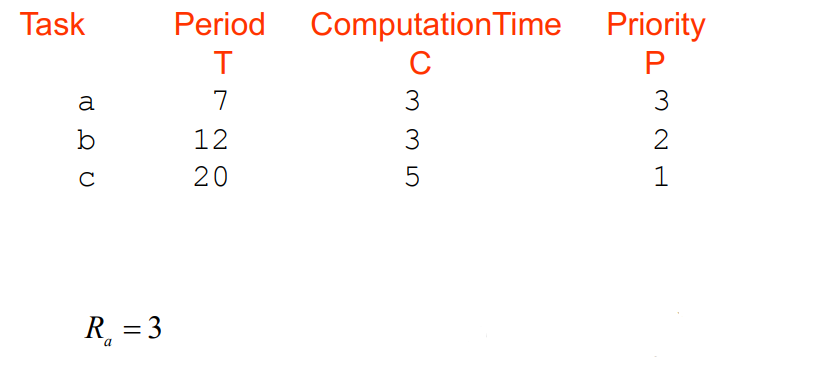
\includegraphics[width=0.9\linewidth]{figures/Scheduling/Response Time Analysis/example.PNG}
\end{figure}
\begin{align}
    w_b^0 = 3 \\
    w_b^1 = 3 + \ceil*{\frac{3}{7}}3 = 6 \\
    w_b^2 = 3 + \ceil*{\frac{6}{7}}3 = 6\\
    R_b = 6
\end{align}
\begin{align}
w_c^0 = 5
w_c^1 = 5 + \ceil*{\frac{5}{12}}3 + \ceil*{\frac{5}{7}}3 = 11 \\
w_c^2 = 5 + \ceil*{\frac{11}{12}}3 + \ceil*{\frac{11}{7}}3 = 14 \\
w_c^3 = 5 + \ceil*{\frac{14}{12}}3 + \ceil*{\frac{14}{7}}3 = 17 \\
w_c^4 = 5 + \ceil*{\frac{17}{12}}3 + \ceil*{\frac{17}{7}}3 = 20 \\
w_c^5 = 5 + \ceil*{\frac{20}{12}}3 + \ceil*{\frac{20}{7}}3 = 20 \\
R_c = 20
\end{align}
We have that for both task a, taks b and task c, $R_i\leq D_i=T_i$ 

\subsubsection{Summary}
Response time analysis is \textbf{sufficient and necessary (exact)}. If the task set passes the test they will meet all their deadlines and if they fail the test then at run-time a task will miss its deadline under the assumption that computation time estimations themselves are not pessimistic)

\subsection{Task Interactions and Blocking}
If a task is suspended waiting for a lower-priority task to complete some required computation then the priority model is in some sense being \textit{undermined}. It is said to suffer \textbf{priority inversion} and the high-priority task waiting for low-priority is said to be \textbf{blocked}. To show this, consider an example where four periodic tasks a,b,c and d and two resources Q and V are at play:
\begin{figure}[H]
    \centering
    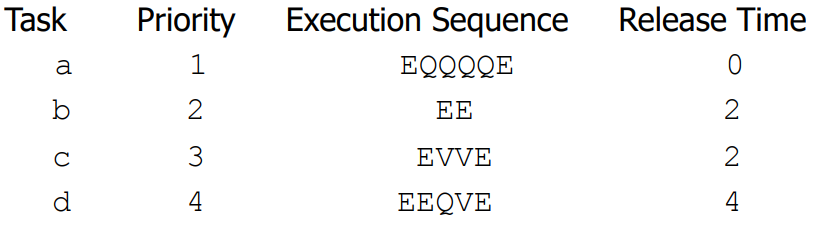
\includegraphics[width=0.9\linewidth]{figures/Scheduling/Priority Inversion/Overview.PNG}
\end{figure}
\begin{figure}[H]
    \centering
    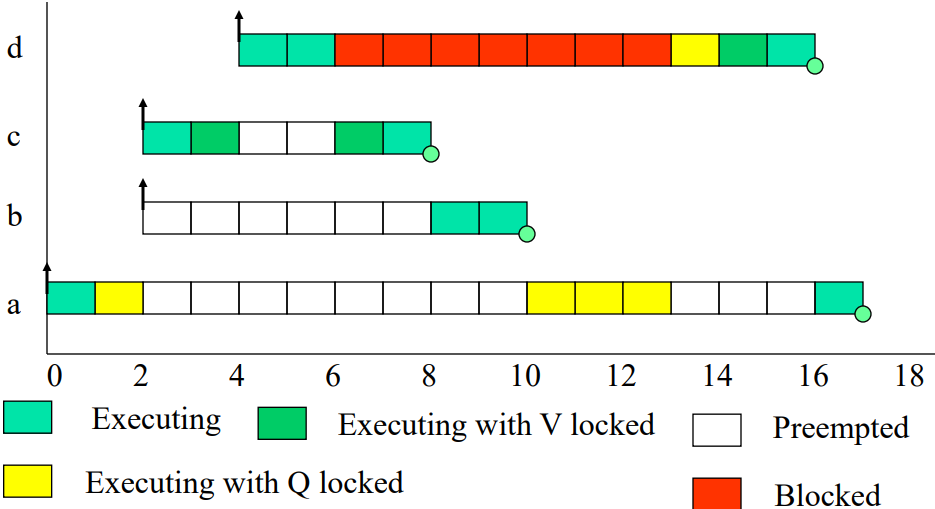
\includegraphics[width=0.9\linewidth]{figures/Scheduling/Priority Inversion/Sequence.PNG}
\end{figure}
What we see here is that if task $p$ is blocking task $q$, then $p$ runs with $q$ 's priority. Above d runs with a's priority.

\subsection{Priority Ceiling Protocols}
A priority ceiling protocol avoids \textbf{unbounded priority inversion} and deadlock. Each shared resource is assigned a ceiling priority equal to the highest priority of any task that can lock it. There are two forms
\begin{itemize}
\item Original Ceiling Priority Protocol (OCPP)
\item Immediate ceiling priority protocol (ICPP)
\end{itemize}
If we are on a single processor, the protocol ensures the following
\begin{itemize}
\item High-priority task can be blocked at most once during its execution by lower-priority tasks.
\item Deadlocks are prevented
\item Transitive blocking is prevented
\item Mutual exclusive access to resources is ensured by the protocol itself.
\end{itemize}

\subsubsection{OCPP}
\begin{itemize}
\item Each task has a static default priority assigned.
\item  Each resource has a static ceiling value defined, this is the maximum priority of the tasks that use it.
\item A task has a dynamic priority that is the maximum of its own static priority and any it inherits due to it blocking higher-priority tasks,
\item A task can only lock a resource if its dynamic priority is higher than the ceiling of any currently locked resource excluding any that it has already locked itself.
\end{itemize}
\begin{figure}[H]
\centering
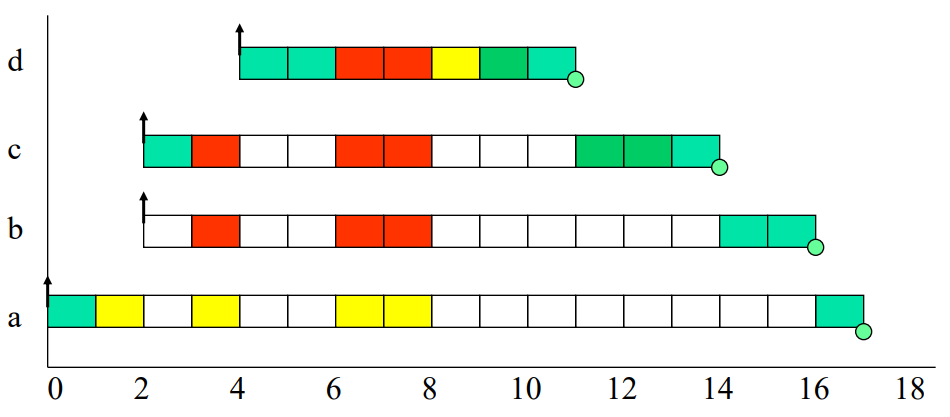
\includegraphics[width=0.9\linewidth]{figures/Scheduling/Priority Inversion/OCPP.PNG}
\end{figure}

\subsubsection{ICPP}
\begin{itemize}
\item Each task static default priority
\item Resource has static ceiling value defined, this is maximum priority of the tasks that use it.
\item A task has a dynamic priority that is the maximum of static and ceiling value of any resource it has locked.
\item Consequence of ICPP; task will only suffer block at the very beginning of its execution.
\item Consequence of ICPP; once task starts executing, all resources it needs must be free; if they were not, then some task would have an equal or higher priority and the task's execution would be postponed.
\end{itemize}
\begin{figure}[H]
\centering
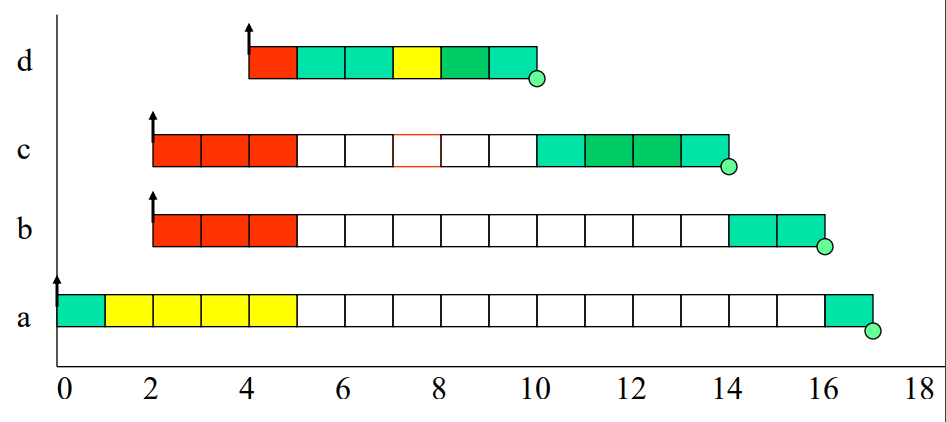
\includegraphics[width=0.9\linewidth]{figures/Scheduling/Priority Inversion/ICPP.PNG}
\end{figure}

\subsubsection{OCPP versus ICPP}
Worst-case behavior is identical but are some differences:
\begin{itemize}
\item ICPP easier to implement as blocking relationships need not be monitored.
\item ICPP leads to less context switching
\item ICPP requires more priority movements as this happens with all resource useage.
\item OCPP changes priority only if an actual block has occurred.
\end{itemize}


\end{document}